\documentclass{beamer}
\usepackage{listings, listings-rust}
\usepackage{graphicx}

\lstset{escapeinside={<@}{@>}}


\usepackage{beamerthemeTUW}
%\usepackage{enumitem}
\setbeamercovered{transparent}


\title{Formally Verifying Rust}
\subtitle{Making sure your Rust code works}
\author{Mark Chimes}
\date{\today}

\begin{document}

\begin{frame}
    \titlepage
\end{frame}

\begin{frame}{Outline}
\tableofcontents
\end{frame}

\section{Rust}
\begin{frame}{Overview}
\begin{block}{What will we do?}
\begin{itemize} 
	\item Introduce Rust
	\item Intrduce Formal verification
	\item Motivate why formally verify with Rust
	\item Examples of Rust Verification
\end{itemize}
\end{block}
\end{frame}


\section{Rust Intro}
\begin{frame}{Rust}
\begin{block}{What is Rust?}
\begin{itemize}
	\item Rust is a \textbf{systems} programming language
	\begin{itemize}
		\item low-level control
		\item fast / efficient
	\end{itemize}
	\item strongly-typed
	\item ``ownership" and ``borrowing"
\end{itemize}
\end{block}
\begin{block}{Special Sauce} 
Memory safety guarantees without garbage collection
\end{block}
\end{frame}


\begin{frame}[fragile]
\frametitle{Ownership and Borrow Examples}
\begin{lstlisting}[language=Rust]
foo(s); // foo takes ownership of s
bar(&t); // bar borrows t as read-only
baz(&mut u); // baz borrows u and can modify it
\end{lstlisting}
\end{frame}


\begin{frame}{Rust: Variable Scopes}
\begin{block}{} 
\begin{itemize}
\item Rust automatically calculates lifetimes
\item When an object goes out of scope, Rust calls its destructor and frees its resources
\item ``Resource Acquisition is Initialization" 
\end{itemize}
\end{block}
\begin{quote}
``resource is guaranteed to be held between when initialization finishes and finalization starts 
and to be held only when the object is alive"
\end{quote}
\end{frame}


\begin{frame}[fragile]
\frametitle{Drop example}


\begin{block}{}
\begin{lstlisting}[language=Rust]
fn create_box() {
    let my_box = Box::new(1i32);
    borrow_box(&my_box);

    // my_box memory freed here
}
\end{lstlisting}

\end{block}
\begin{lstlisting}[language=Rust]
fn borrow_box(ibox: &Box<i32>)
\end{lstlisting}
\end{frame}


\begin{frame}{Borrowing}
\begin{block}{Rust Ownership and Borrowing}
\begin{itemize} 
	\item One owner
	\item One read/write borrow
	\item Multiple read-only borrows
	\item When lifetime ends, item is returned
\end{itemize} 
\end{block}
\end{frame}

\begin{frame}[fragile]
\frametitle{Multiple Borrows Example}
\begin{block}{}
\begin{lstlisting}[language=Rust]
    let mut s = String::from("hello");
    
    let t1: &mut String = &mut s;
    // <@\textcolor{blue}{t1 never used again, gets dropped}@>
    let t2: &mut String = &mut s;

    let len = calculate_length(t2);
 \end{lstlisting}
\end{block}
\begin{lstlisting}[language=Rust]
fn calculate_length(s : &String) -> usize
\end{lstlisting}
\end{frame}


\begin{frame}[fragile]
\frametitle{Not Fine}
\begin{block}{}
\begin{lstlisting}[language=Rust]
    let mut s = String::from("hello");
    
    let t1: &mut String = &mut s;
    // <@\textcolor{red}{t1 used again later, still active}@>
    let t2: &mut String = &mut s;

    let len = calculate_length(<@\textcolor{red}{t1}@>); // fails
 \end{lstlisting}
\end{block}
\begin{lstlisting}[language=Rust]
fn calculate_length(s : &String) -> usize
\end{lstlisting}
\end{frame}




\begin{frame}{Unsafe Rust}
\begin{block}{Unsafe Rust}
\begin{itemize} 
	\item it also exists
\end{itemize} 
\end{block}
\end{frame}


\section{Formal Verification Intro}
\begin{frame}{Formal Verification}
\begin{block}{What is Formal Verification?}
\begin{itemize} 
	\item Program verification: Logically ``prove" correctness of a program
	\item labour-intensive process
	\item Can involve manual encoding in e.g. Roq (Coq), Agda, Lean, Idris
	\item Some tools for (partial) automation: Dafny, Viper, etc.
	\item Often rely on an SMT solver and/or Horn Clause solver
	\item ``very high level of reliability" BUT only as good as your mathematical model 
	\item Other methods (e.g. model checking) also exist.
\end{itemize} 
\end{block}
\end{frame}


\begin{frame}
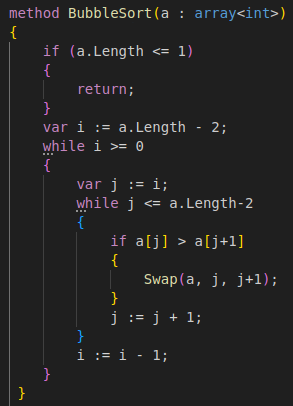
\includegraphics[scale=0.6]{pictures/verification/bubblesort.png}
\end{frame}

\begin{frame}
\begin{center}
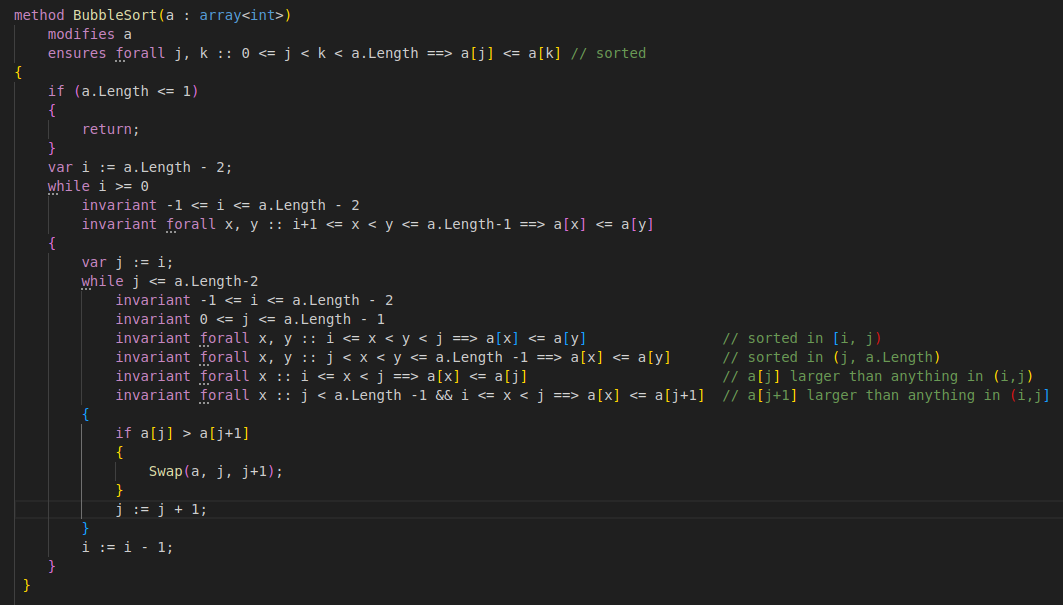
\includegraphics[scale=0.3]{pictures/verification/bubblesort_annotated.png}
\end{center}
\end{frame}

\section{Combination}
\begin{frame}{}
\begin{center}
What makes Rust interesting for Verification?
\end{center}
\end{frame}


\begin{frame}[fragile]{Aliasing Problem}
Two pointers
\begin{block}{C program}
\begin{lstlisting}[language=C]
void increment_both(int *x, int *y)
{
    *x = *x + 1; 
    *y = *y + 1;   
}
 \end{lstlisting}
\end{block}

Want to prove after ``increment both" is done, that\\
x\_end = x\_start + 1 and \\
y\_end = y\_start + 1

\end{frame}

\begin{frame}[fragile]{Aliasing Problem}
\begin{block}{C program}
\begin{lstlisting}[language=C]
void increment_both(int *x, int *y)
{
    *x = *x + 1; 
    *y = *y + 1;   
}
 \end{lstlisting}
\end{block}

\begin{block}{Calling ``increment both" with same variable twice}
\begin{lstlisting}[language=C]
int a = 0;
increment_both(&a, &a); 
\end{lstlisting}
\end{block}
\end{frame}

\begin{frame}{Proof Difficulty}
\begin{itemize}
\item
Aliasing could happen anywhere in the program
\item
Correct usage of increment\_both relies on \emph{non-local} information!
\item
Strategies exist, involving e.g. separation logic
\item But in Safe Rust, mutable references can \emph{never alias}
\item Rust also strongly typed, and borrows must be marked read / write
\end{itemize} 
\end{frame}



\begin{frame}[fragile]
\begin{block}{C program}
\begin{lstlisting}[language=C]
const char *msg = "hello, world!"; 
int len = get_length(msg);
// do something else with msg
\end{lstlisting}
\end{block}

\begin{block}{Rust program}
\begin{lstlisting}[language=rust]
let msg = "hello, world!"; 
let len = get_length(&msg);  
// do something else with msg
\end{lstlisting}
\end{block}


in C, must add conditions that get\_length does not modify 
msg

but in Rust, msg is not mutable
\end{frame}

\begin{frame}{Unsafe Rust} 
\begin{itemize}
\item 
Unsafe Rust is essential for functioning of Rust 
\item 
It is more difficult to verify since we do not have the safety guarantees \emph{inside} unsafe blocks
\item 
But we can still isolate (un)safety, make assumptions, prove separately
\end{itemize} 
\end{frame} 

\section{Rust Verifiers}

https://docs.google.com/document/d/1toq2g81wjf27UohWYZBSptEX5R1NnIgshVAwFxO94kM/edit?tab=t.0

https://chatgpt.com/c/685973b6-8c08-8007-b81a-515cafb07605

\begin{frame}{Rust Verification Tools}
\begin{itemize} 
\item Prusti (Viper)
\item Flux
\item Creusot
\item RustHorn
\item RustHornBelt
\item Aeneas
\item Gilian-Rust
\end{itemize} 
\end{frame}

\begin{frame}{Prusti} 

\end{frame}

\end{document}
